\chapter{Repozytorium i system kontroli wersji}

GitHub to platforma do udostępniania projektów programistów a nawet projektów całych zepsołów programistków. Oferuje wiele narzedzi umożliwiających pracę z projektem i zarządzaniem ich kodami. Jest on raczej jednym z popularniejszych stron hostujących projekty innych osób. Można tam dodać pliki jak i je pobierać i dowolnie edytować. Pliki do projektu zostały umieszczone w repozytorium pod adresem https://github.com/ErwinKisiel/SystemZarzadzaniaKontemKlienta.git.

\begin{figure}[h]
    \centering
    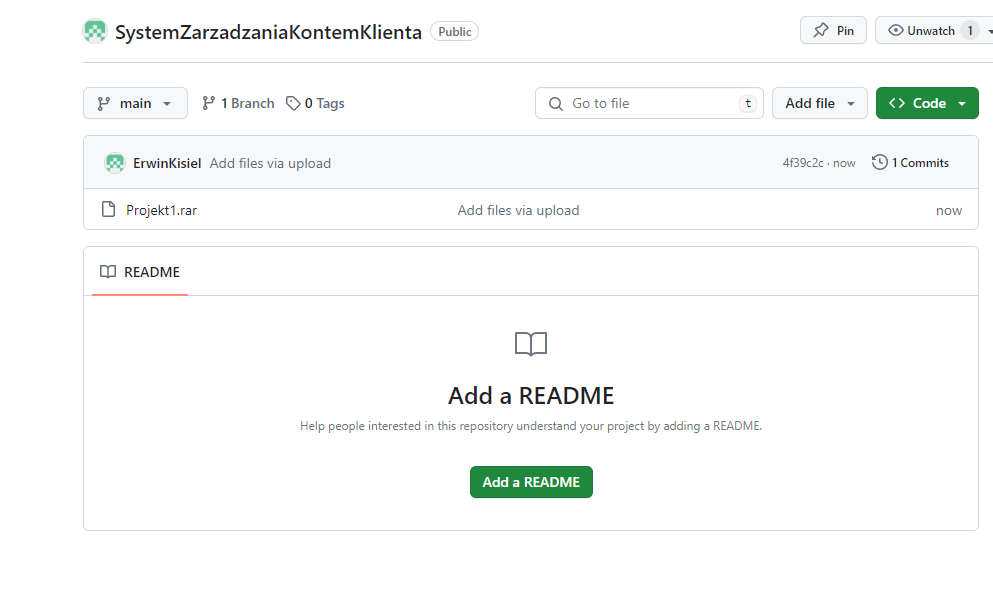
\includegraphics[width=\textwidth]{Repozytorium.png}
      \caption{Repozytorium na GitHub}
    \label{fig:example}
\end{figure}
